\documentclass[11pt,a4paper]{report}
\usepackage{amsmath}
\usepackage{amsfonts}
\usepackage{amssymb}
\usepackage{setspace}
\usepackage{url}
%\usepackage{cite}
\usepackage{fancyhdr}
\usepackage{titlesec}
\titleformat{\subsection}{\itshape\normalsize}{\thesubsection}{1em}{}
% interligne
\usepackage{pdflscape}
\usepackage{placeins}
\usepackage{cite}
\usepackage[left=2cm,
			right=2cm,
			top=3cm,
			bottom=3cm]{geometry}
\author{Cyril Matthey-Doret}
\usepackage{outline} \usepackage{pmgraph} \usepackage[normalem]{ulem}
\usepackage{verbatim}
\pagestyle{fancy}
\setlength{\footskip}{80pt}
% chargement des figures
\usepackage{graphicx}					
\usepackage{wrapfig}
\usepackage[export]{adjustbox}
\usepackage{caption}

\title{

\includegraphics[width=1.75in]{lo_unil06_bleu.pdf} \\
\vspace*{1in}
\textbf{Do enhancer-associated lincRNAs contribute to chromosomal organization ?}}

\author{\Large{First Step Project}\\
		Molecular Life Sciences, Bioinformatics\\
				\vspace*{0.5in} \\
		Cyril Matthey-Doret\\
        Supervised by: Jennifer Yihong Tan\\
        Directed by: Ana Claudia Marques\\
		\vspace*{0.5in} \\
		Department of Computational Biology\\
		Department of Physiology\\
        \textbf{University of Lausanne - Switzerland}\\
       } \date{\today}
%--------------------Make usable space all of page
\setlength{\oddsidemargin}{0in} \setlength{\evensidemargin}{0in}
\setlength{\topmargin}{0in}     \setlength{\headsep}{+0.5in}
\setlength{\textwidth}{6.5in}   \setlength{\textheight}{8.5in}
%--------------------Indention
\setlength{\parindent}{1cm}

\begin{document}

%--------------------Title Page
\renewcommand{\headrulewidth}{1pt}
\fancyhead[R]{First Step Project, University of Lausanne - Switzerland, December 2016}
\maketitle
%--------------------Begin Outline

\section*{Abstract}

A large proportion of the human genome generates RNA that is not translated into proteins, denoted as noncoding RNA. Long noncoding RNAs (lncRNAs), are longer than 200 nucleotides and represent the largest part of the noncoding transcriptome in humans, outnumbering protein-coding genes by almost 3 times. Although less than 1\% of these transcripts have been functionally annotated, a wide array of regulatory functions have already been attributed to lncRNAs. In particular, it has recently been found that intergenic lncRNAs (lincRNAs) associated with human trait variants often arise from enhancer transcription and coindide with regions of high frequencies of chromosomal contacts. There are already some characterized enhancer-associated lincRNAs (elincRNAs) known to regulate these chromosomal contacts, but whether this is a general function of elincRNAs or these are just isolated cases is unknown. Modulation of chromosomal architecture, for example by establishing loops or highly compact regions called topologically associated domains (TADs), is crucial for regulation of gene expression, allowing correct interactions between enhancers and promoters. Here, I investigate the role of these elincRNAs in spatial organization of the genome in a human lymphoblastoid cell line, making use of functional genomics and data from recent advances in chromosome conformation capture techniques that allow to quantify DNA:DNA contacts genome wide (Hi-C).

\section*{Introduction}
It was only discovered in the past decade that a surprisingly large proportion of the mammalian transcriptome does not code for proteins. To date, the number of annotated noncoding genes longer than 200 nucleotides (long noncoding RNA, lncRNA) exceeds that of protein-coding genes by at least 3 times \cite{Iyer2015}⁠. Among lncRNAs, those that do not overlap protein-coding genes are the most abundant, referred to as long intergenic noncoding RNAs, lincRNAs. Functional and evolutionary analyses, together with extensive characterization of a handful of lincRNAs, demonstrate that some of these transcripts are involved in the regulation of gene expression programs, both transcriptionally and post-transcriptionally, and that they can contribute to organismal traits and diseases \cite{Kornienko2013}⁠. However, the mechanisms and functions, if any, for the majority of lincRNAs remain unknown \cite{Rinn2012}⁠.  

A high proportion of lincRNA arise from enhancers, as most active enhancers are transcribed, generating noncoding products, including lincRNAs \cite{Guil2012}. Recently, lincRNAs associated with human trait variants have been shown to have enhancer-associated cis-regulatory roles on local gene expression. Importantly, these loci are correlated with higher frequencies of chromosomal interactions relative to other lincRNAs in a human lymphoblastoid cell line (LCL), suggesting that enhancer-associated lincRNAs (elincRNAs) may be involved in gene regulation through modulating chromatin architecture (Tan et al, 2016, under revision). 

Indeed, spatial organization of the genome impacts gene regulation \cite{Engreitz2016}⁠⁠. Specifically, the folding of genomic DNA into variably compact chromosomal structures can strongly influence expression of the embedded genes \cite{Gorkin2014}⁠⁠. Globally, regions with low degree of compaction are associated with high levels of active transcription, referred to as euchromatin. On the other hand, relatively uncondensed and less transcriptionally active regions are called heterochromatin \cite{Passarge1979}\cite{Tamaru2010}⁠. Chromosomes are further compartmentalized into smaller domains where frequent DNA:DNA interactions occur as a result of their close spatial proximity, called topologically associating domains (TADs), which are key in modulating gene transcription programs. Recent findings show that regions at the borders of TADs, called TAD boundaries, are essential for modulating and preventing gene regulatory interactions within and across TADs, respectively. Deletion of TAD boundaries often disrupts those interactions, resulting in gene misexpression and disease phenotypes \cite{Lupianez2015}⁠.

Detailed functional characterization of some elincRNAs have demonstrated the molecular mechanisms underlying their roles in the spatial organization of the genome. For example, Haunt is one such elincRNA \cite{Yin2015}⁠⁠, which can regulate expression of the HOXA gene cluster by modulating intrachromosomal interactions, specifically through promoter-enhancer looping. These recent findings raise the question on what is the prevalence of elincRNAs contributing to gene regulation through modulation of chromosomal conformation.

Using various bioinformatics tools to analyze publicly available multi-omics data from human lymphoblastoid cell lines (LCLs). I investigated the molecular properties of elincRNAs. Specifically, I examined their enrichment in regions that are key in TAD regulation and their association with the amount of chromosomal interactions to gain initial insight into their roles in gene regulation within topological domains. My analyses show that elincRNAs are associated with high density of DNA:DNA contacts within TADs and are significantly enriched in protein binding sites important for TAD regulation. Importantly,  elincRNAs are strongly enriched at chromosomal loop anchors where promoter-enhancer interactions occur, supporting the hypothesis that they may contribute to gene regulation by establishing contacts between gene regulatory elements and modulating chromosomal organization.
\section*{Results}

Enhancer-associated lincRNAs (elincRNAs) in human lymphoblastoid cell lines (LCLs) were identified based on overlap with LCL enhancers predicted from histone marks (GM12878, \cite{ENCODEProject2012}⁠) at their putative promoter regions, estimated as 1kb upstream from their transcriptional start site. LincRNAs whose promoter region also overlapped other predicted regulatory regions, specifically promoter elements \cite{ENCODEProject2012}⁠, in LCLs were excluded from the analysis (elincRNAs=236, other LCL-expressed lincRNAs=1756).

\subsection*{elincRNAs show similar expression levels as other lincRNAs}

Unlike most enhancer-associated noncoding RNAs (eRNAs) which are often transcribed bidirectionally and then rapidly degraded by the nuclear exosome \cite{Darrow2013} \cite{Lam2014}⁠, elincRNAs are more stably and preferentially transcribed in one direction, and are often spliced and polyadenylated \cite{Marques2013a}⁠. 
First, to investigate if LCL-expressed elincRNAs share similar expression profiles as the lowly expressed eRNAs relative to other expressed genes, I compared  expression levels of elincRNAs to that of other lincRNAs and protein-coding genes (Figure \ref{charac_elinc}A). I found that elincRNAs are not more lowly expressed compared to other lincRNAs in human LCLs (GM12878, two-tailed Mann-Whitney U test, $p=0.258$), suggesting elincRNAs may have distinct properties compared to other enhancer-associated transcripts.

\subsection*{elincRNA transcripts are less conserved than other lincRNAs}

To gain insights into elincRNAs evolution, I investigated the nucleotide conservation of their exons in primates and placental mammals using phastCons scores \cite{Siepel2005}⁠, as a measure of nucleotide conservation (Methods). I found that exons of elincRNAs are less conserved than other LCL-expressed lincRNAs (two-tailed Mann-Whitney U test, mammals: $p<1e-07$, primates: $p<1e-05$) as well as  protein coding genes (two-tailed Mann-Whitney U test, mammals: $p<1e-97$, primates: $p<1e-86$) (Figure \ref{charac_elinc}C). 

Interestingly, recent studies on a set of trait-relevant and enhancer-associated lincRNAs showed that although exons of these lincRNAs did not seem to have evolved under purifying selection relative to other LCL-expressed lincRNAs across mammalian and primate evolution, their sequences are constraint specifically during recent human evolution (Tan et al, 2016, under revision). Therefore, although my result may suggest that elincRNA transcripts were not evolving under constraint across broad mammalian evolution, their conservation across modern human evolution remains to be investigated.

\subsection*{elincRNAs promoter regions are enriched at loop anchors and cohesin binding}

Next, to examine whether elincRNAs are associated with the regulation of chromosomal architecture, I investigated the co-localization of elincRNAs with regulatory regions essential in establishing chromosomal interactions within topologically associating domains (TADs). Specifically, significant enrichment ⁠of elincRNAs, compared to what would be expected if they were randomly distributed across the intergenic regions of the genome (Methods), was found at loop anchors (fold enrichment = 2.79, $q=1e-04$, Figure \ref{enrich_elinc}A), where enhancer-promoter gene regulatory interactions occur \cite{Ji2016}.  

Previous studies have demonstrated that regulatory proteins are also enriched at the loop anchors within TADs \cite{Rao2014}⁠. Specifically, the cohesin protein-complex has been previously shown to be important for intra-TAD gene regulation in a cell type-specific manner \cite{Hadjur2009}⁠. Also enriched at loop anchors, the CTCF transcription factor is another central player in the regulation of chromatin architecture and gene expression. According to a recent model \cite{Ji2016}⁠, loops mediated by CTCF or CTCF and cohesin collectively have insulating properties, preventing interactions across TADs and are important for the structural maintenance of TADs. In contrast, loops containing only cohesin binding sites are crucial in mediating regulatory chromosomal interactions. Cohesin depletion is associated with disrupted promoter-enhancer interactions within TADs \cite{Seitan2013}⁠.

Significant enrichments were found for CTCF and cohesin binding peaks (subunits, SMC3 and RAD21 are used to measure cohesin binding, methods) within elincRNAs promoter regions (fold enrichment = 5.2 and 8.1, respectively, $q=1e-04$) relative to other lincRNAs (fold enrichment = 1.3 and 1.3, respectively, $q<0.05$, Figure \ref{enrich_elinc}C).

As most binding sites for CTCF and cohesin overlap in the human genome (Figure \ref{enrich_elinc}E) and loops mediated by CTCF or cohesin independently, or both CTCF and cohesin collectively are thought to have different roles in chromosomal organization \cite{Ji2016}⁠, I further determined the independent enrichment of elincRNAs in CTCF and cohesin binding by obtaining mutually exclusive binding sites of the proteins. This revealed a much stronger enrichment of cohesin binding sites (Figure \ref{enrich_elinc}D) in elincRNA loci (fold enrichment = 13.1, $q=1e-04$) compared to CTCF binding sites (fold enrichment = 3.92, $q=1e-04$). This suggests elincRNAs may be much more frequently involved in the formation of cohesin-only loops, supporting their roles in modulating promoter-enhancer looping.

\subsection*{elincRNAs promoter regions are not enriched at TAD boundaries}

As loop anchors are frequently found at TAD boundaries, I next investigated whether similar enrichment would be observed for elincRNAs at TAD boundaries. Using Hi-C data (Figure \ref{TAD_loop_def}) I estimated TAD boundary regions through a sliding diamond approach on contact matrices (Figure \ref{interact_hic}A, methods). Boundaries were extended from TAD borders until the sum of interactions in the diamond reached an arbitrary threshold (Figure \ref{boundary_ex}, methods). Although elincRNAs promoter regions are enriched at loop anchors relative to other LCL-expressed lincRNAs, no significant enrichment was found for these loci  at TAD boundaries (fold enrichment = 1.2, $q=0.08$, Figure \ref{enrich_elinc}B). Despite the absence of significant elincRNA enrichment at TAD boundaries, dividing TADs into 10 equally sized bins reveals that elincRNAs tend to be more frequently found near the end of the TADs and are depleted at the center of the TADs (bin 5, fold enrichment = 0.37, $q=0.06$) relative to other LCL-expressed lincRNAs (Figure \ref{enrich_elinc}F). The trend is consistent with their enrichment at loop anchors, which are enriched at TAD boundaries (fold enrichment =1.74 , $q<1e-3$, not shown).

This observed lack of significant enrichment  of elincRNAs at TAD boundaries may be a consequence of poor resolution of the current Hi-C technology, which is restrained to a maximum of 5kb \cite{Rao2014}⁠, as well as limitations in the method used to define boundary regions. Particularly, I defined TAD boundaries by extending inwards from borders of TADs (see methods for details), therefore all genes located outside of defined TADs but close to a TAD border are excluded from the analysis. 


\subsection*{elincRNAs are associated with high DNA:DNA contacts within TADs}

To further support their role in regulating promoter-enhancer contacts, I investigated whether elincRNAs are associated with regions with higher DNA:DNA interactions. To this end, I measured the average amount of contact in their respective TADs (Figure \ref{interact_hic}B, methods). I found that elincRNAs are frequently embedded within TADs with higher density of contacts compared to other lincRNAs in GM12878 (Median fold difference=1.24, two-tailed Mann-Whitney U test, $p<1e-04$, Figure \ref{TAD_TAD_contacts}). In addition, fold difference in the amount of DNA contacts within TADs harbouring these elincRNA loci were less pronounced in 3 other cell lines relative to other LCL-expressed lincRNAs (Median fold difference=1.05, 1.07, and 1.04, p=$0.02, 0.04, 0.472$ in HUVEC, K562 and NHEK, respectively) compared to GM12878. This provides evidence that the association between elincRNA expression and chromosomal contacts is likely cell line-dependent. 
Although my findings do not provide insights into the mechanisms through which elincRNAs may regulate chromosomal architecture, their associated high DNA:DNA contacts, together with their enrichment of cohesin binding suggest a role for elincRNAs in the modulation of promoter-enhancer looping within topologically associating domains.

\section*{Figures, tables and legends}

\begin{figure}[ht]
	%\centering
	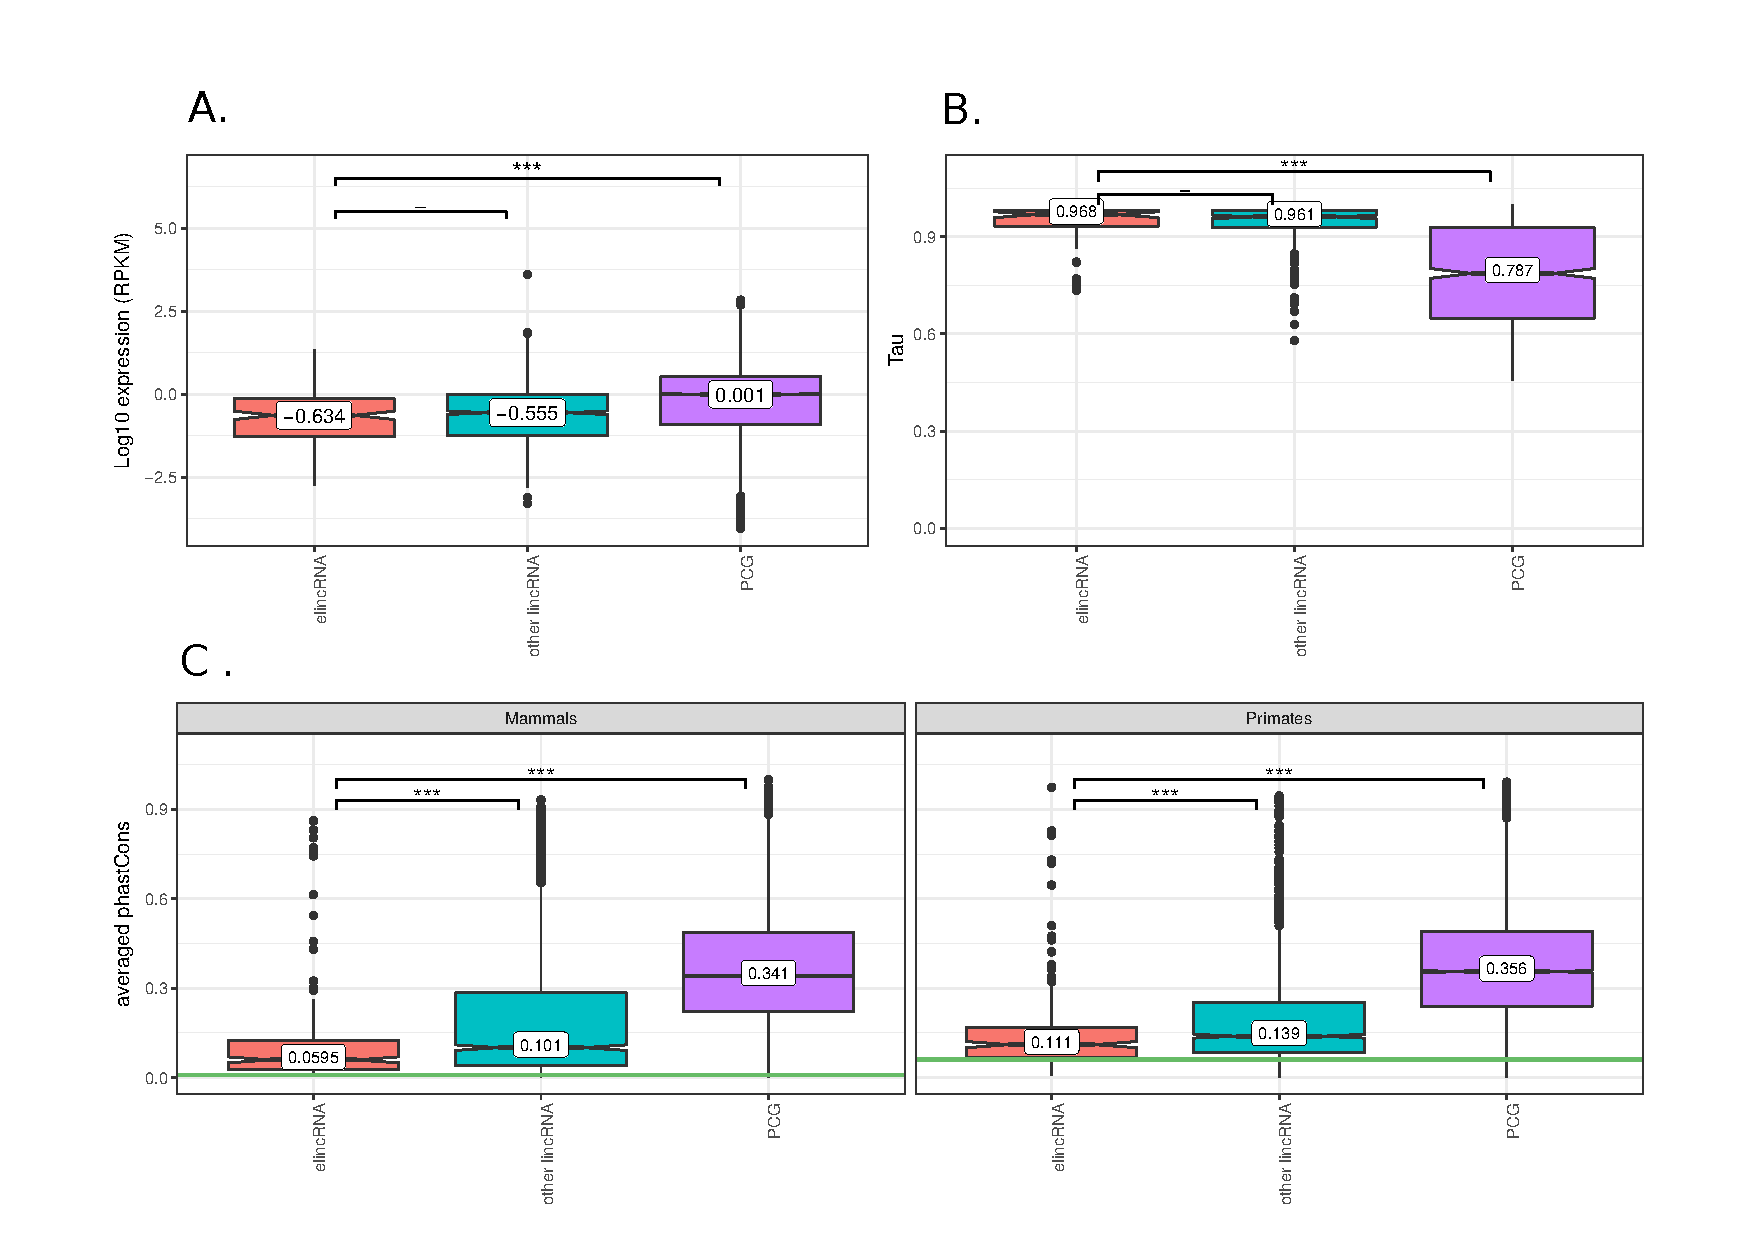
\includegraphics[width=1\textwidth]{Figures/1_full_characterization_elincRNA.pdf}
	\caption{Characteristics of elincRNAs compared to other lincRNAs and protein-coding genes (PCG). Median values are displayed in the boxes. All tests are two-tailed Mann-Whitney test, $***P<0.001$; - not significant. A. Median expression levels in GM12878. B. Tissue specificity index (Tau). The index can take values between 0 (low specificity) and 1 (high specificity). C. Sequence conservation of exons through mammalian and primate evolution. Averaged phastCons score is used as a measure. The green horizontal line represents the median conservation of ancestral repeats, which are assuming to be evolving neutrally. }
	\label{charac_elinc}
\end{figure}

\begin{figure}[ht]
	%\centering
	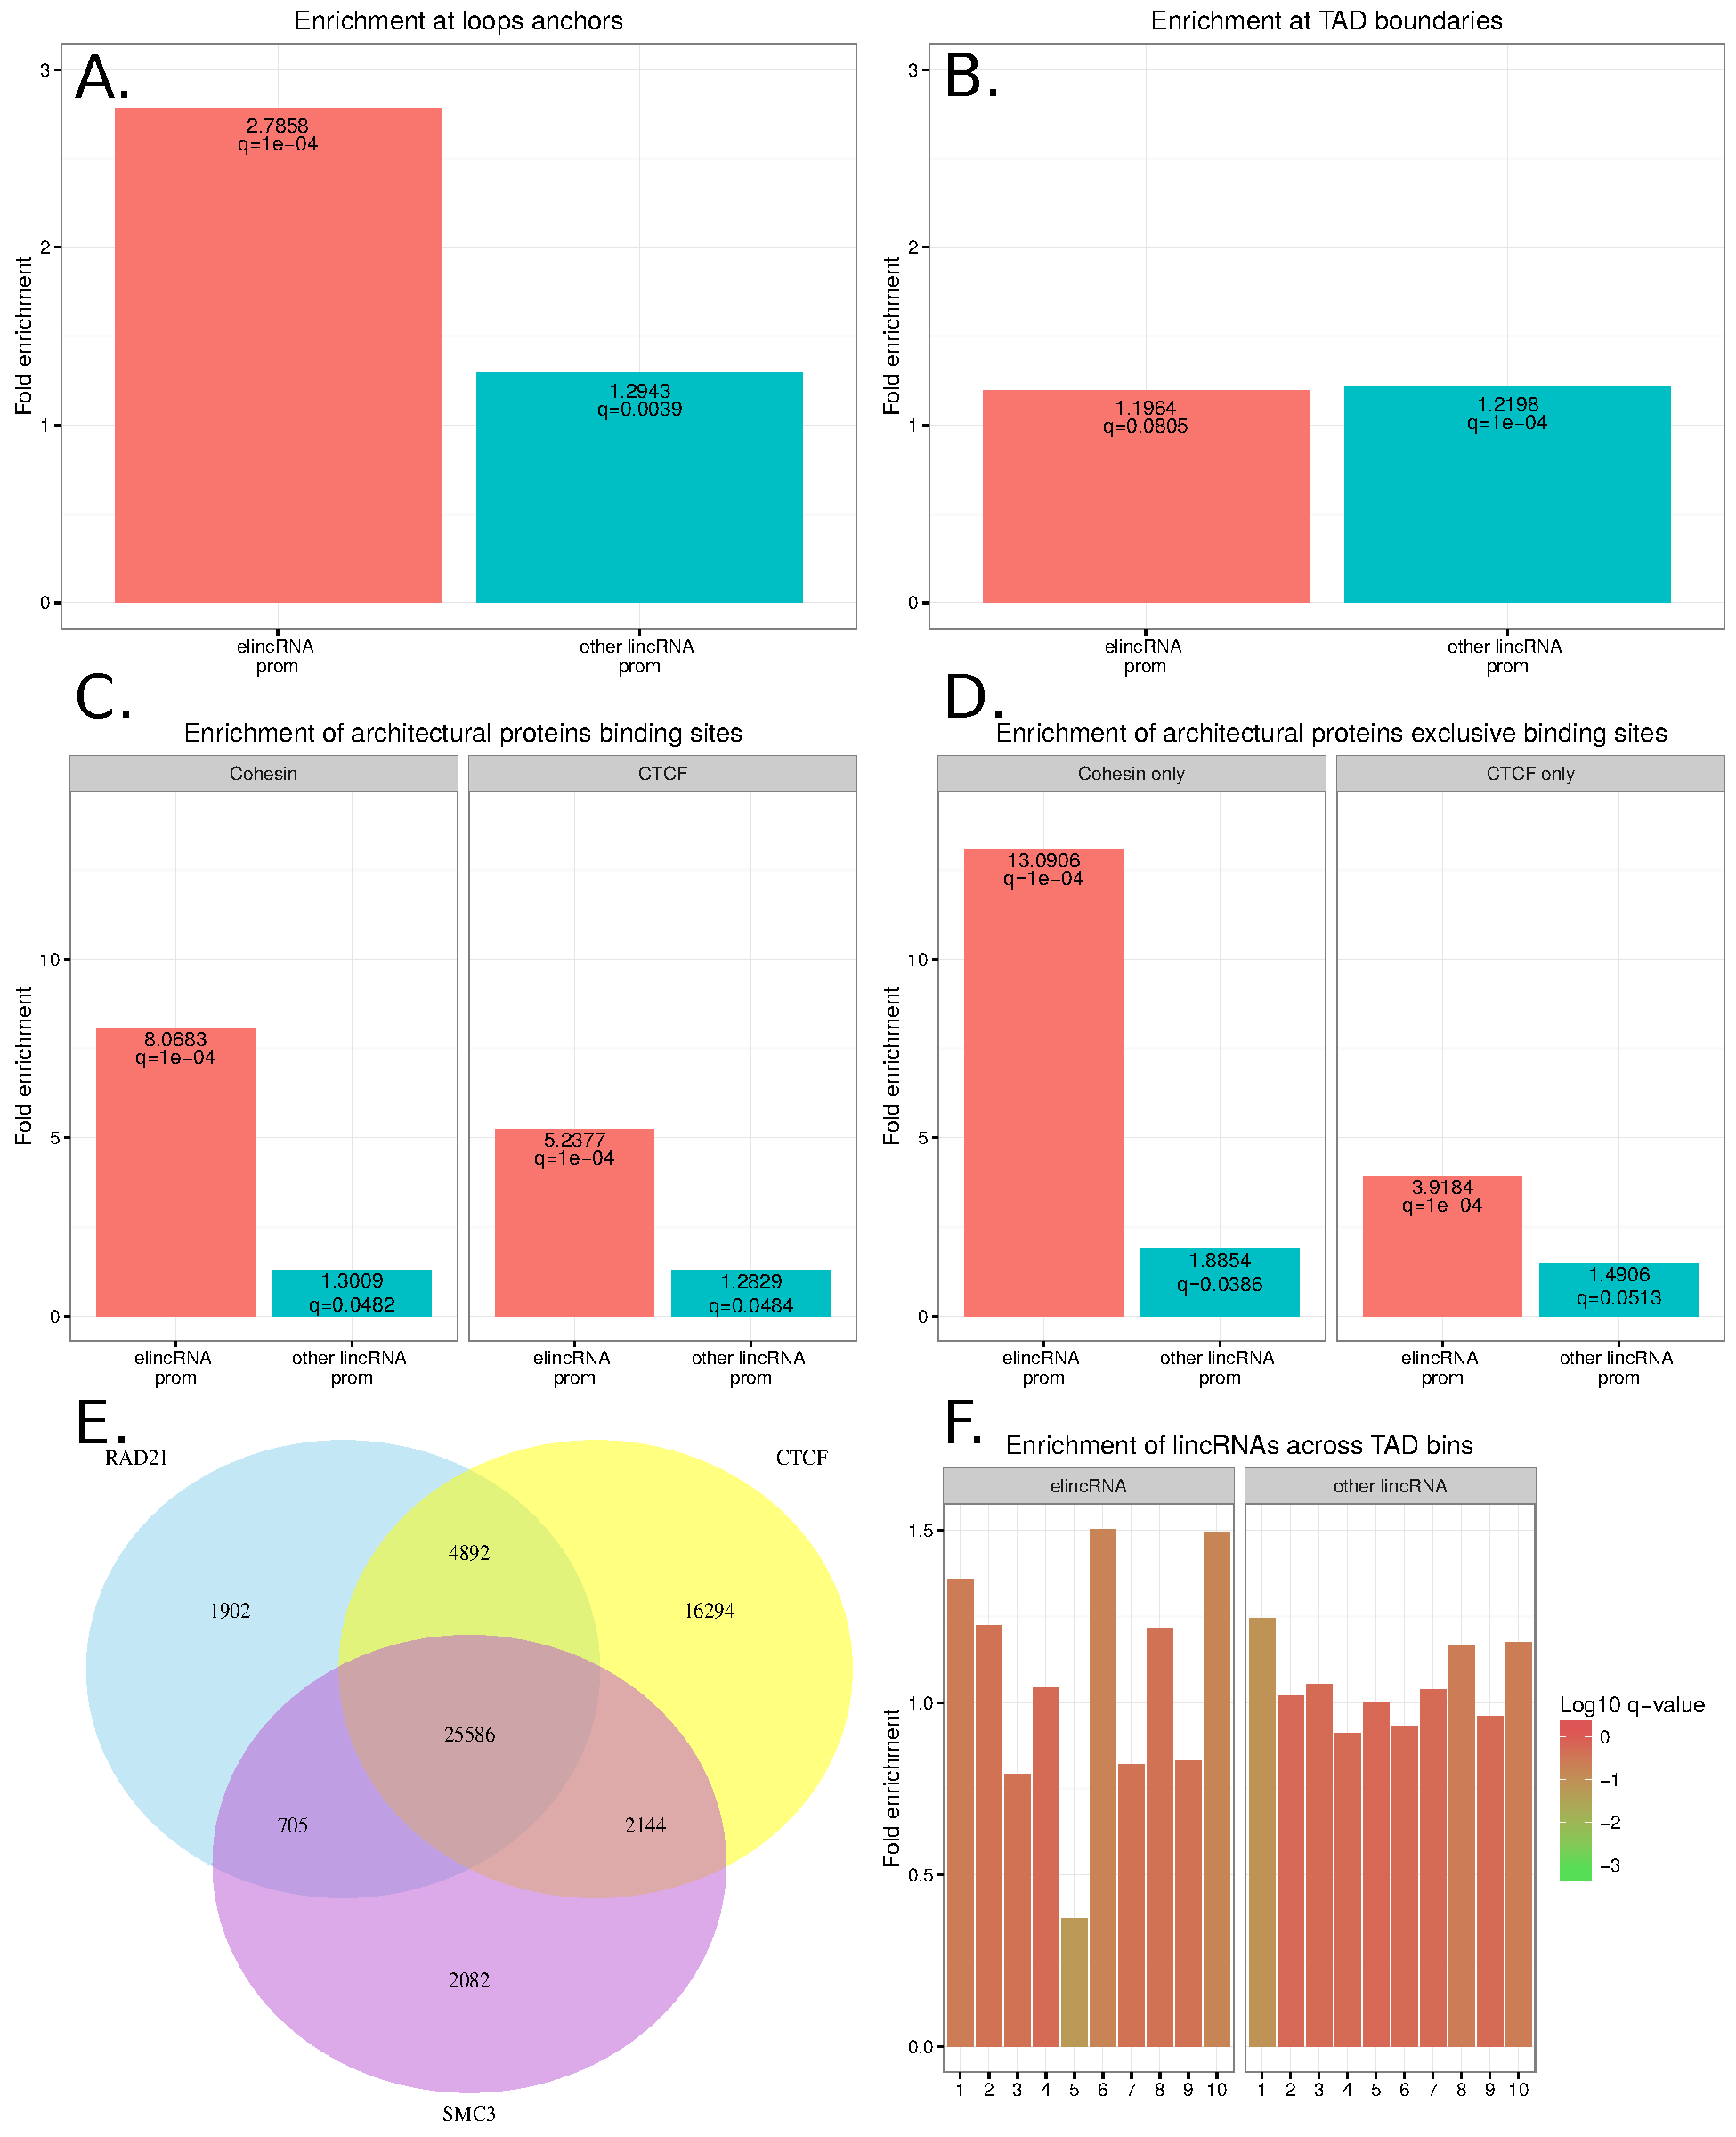
\includegraphics[width=0.9\textwidth]{Figures/2_Enrichment.pdf}
	\caption{Results from GAT enrichment tests. Values displayed on the bars are fold enrichment compared to random expectation, q represents the p-value adjusted for multiple testing using FDR (methods). A. Enrichment of elincRNA promoter regions at loop anchors compared to other lincRNAs. B. Enrichment of elincRNA promoter regions at TAD boundaries compared to other lincRNAs. C. Enrichment in peaks of architectural proteins cohesin and CTCF in elincRNA promoter regions, compared to other lincRNA. D. Enrichment of CTCF and cohesin exclusive binding sites in promoter regions of elincRNAs compared to other lincRNAs. E. Proportions of overlap between RAD21, SMC3 and CTCF peaks in the human genome. F. Enrichment of elincRNAs across TADs compared to other lincRNAs. Each bar represent a bin of 10\% TAD length. The log10 of q-values are put in color codes to give an estimation of the confidence in each value.}
	\label{enrich_elinc}
\end{figure}

\begin{figure}[ht]
	%\centering
	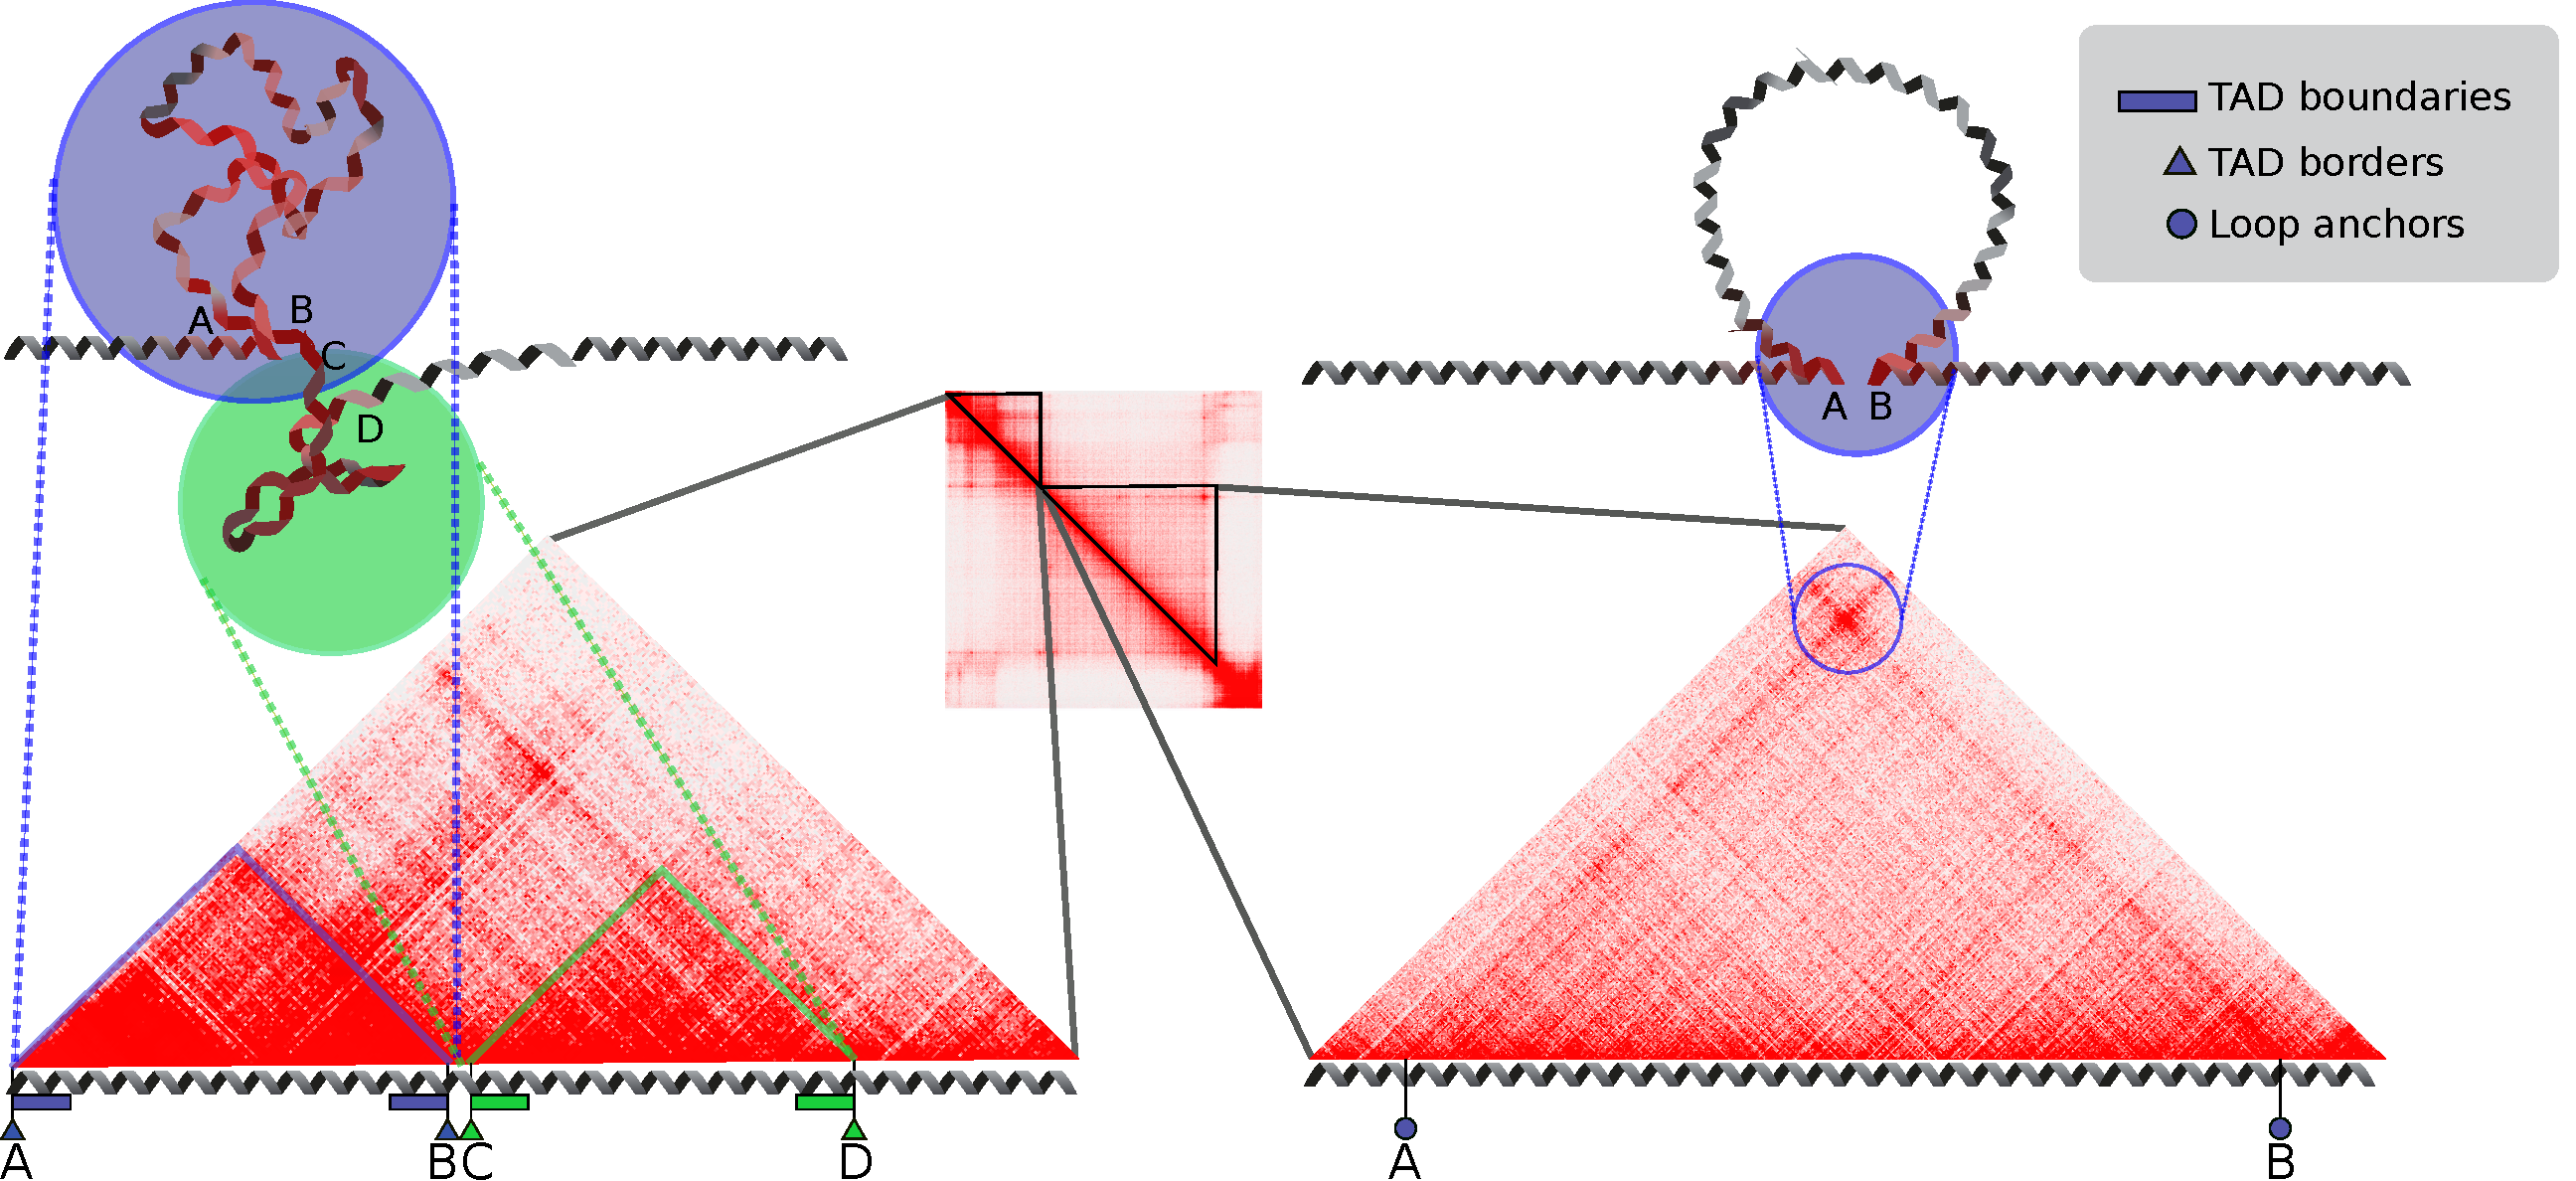
\includegraphics[width=1\textwidth]{Figures/3_TAD_loop_definition.pdf}
	\caption{Schematic representation of TADs and loops and typical patterns  observed in Hi-C matrices corresponding to these structures. Center:  Example of a Hi-C matrix visualized in Juicebox (Durand et al., 2016)⁠. These matrices are symmetric and only upper/lower triangles are therefore used to simplify the visualization. The darker pixels on the matrix contain more interactions. Left: Two separate TADs are observed as high interactions triangle on the matrix. These are examplified by regions of compacted DNA where frequent interactions occur, while interactions across TADs (i.e. between the blue and green triangles) are less frequent. A and B are the borders of the first TAD while C and D are the borders of the second TAD. Boundaries are the rectangles expanding inwards from the borders. Right: Representation of a loop with A and B being the anchors of the loop where strong contact is observed. Unlike TADs, the contact is not particularly high in the region between the two anchors, therefore loops are seen as a sharp increase in contacts deviating from the matrix diagonal. }
	\label{TAD_loop_def}
\end{figure}

\begin{figure}[ht]
	%\centering
	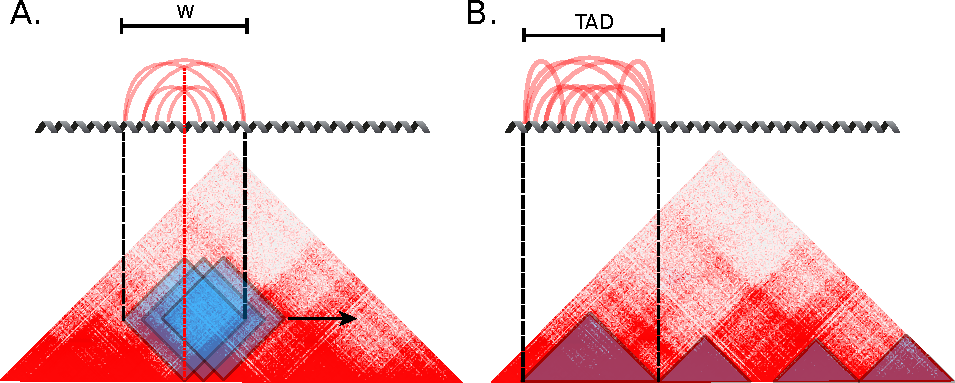
\includegraphics[width=1\textwidth]{Figures/4_interactions.pdf}
	\caption{Visual representations of the algorithms used to compute contacts in Hi-C matrices. As they are symmetric, matrices are represented as upper triangles for simplicity reasons. A: Schematic representation of the algorithm used to measure insulation. A diamond (blue) of width w set to 100kb is slid on all position along the diagonal. For each position, the sum in the diamond is computed and later used to define boundaries. The sum in the diamond at position d (dotted line) represents a measure of all interactions across position d (i.e. between elements before and after position d). B: Method used to compute the mean of all interactions in TADs. Each TAD is taken as a submatrix (upper triangles of the submatrices are depicted in blue) and the mean value in the submatrix is computed. }
	\label{interact_hic}
\end{figure}

\begin{figure}[ht]
	%\centering
	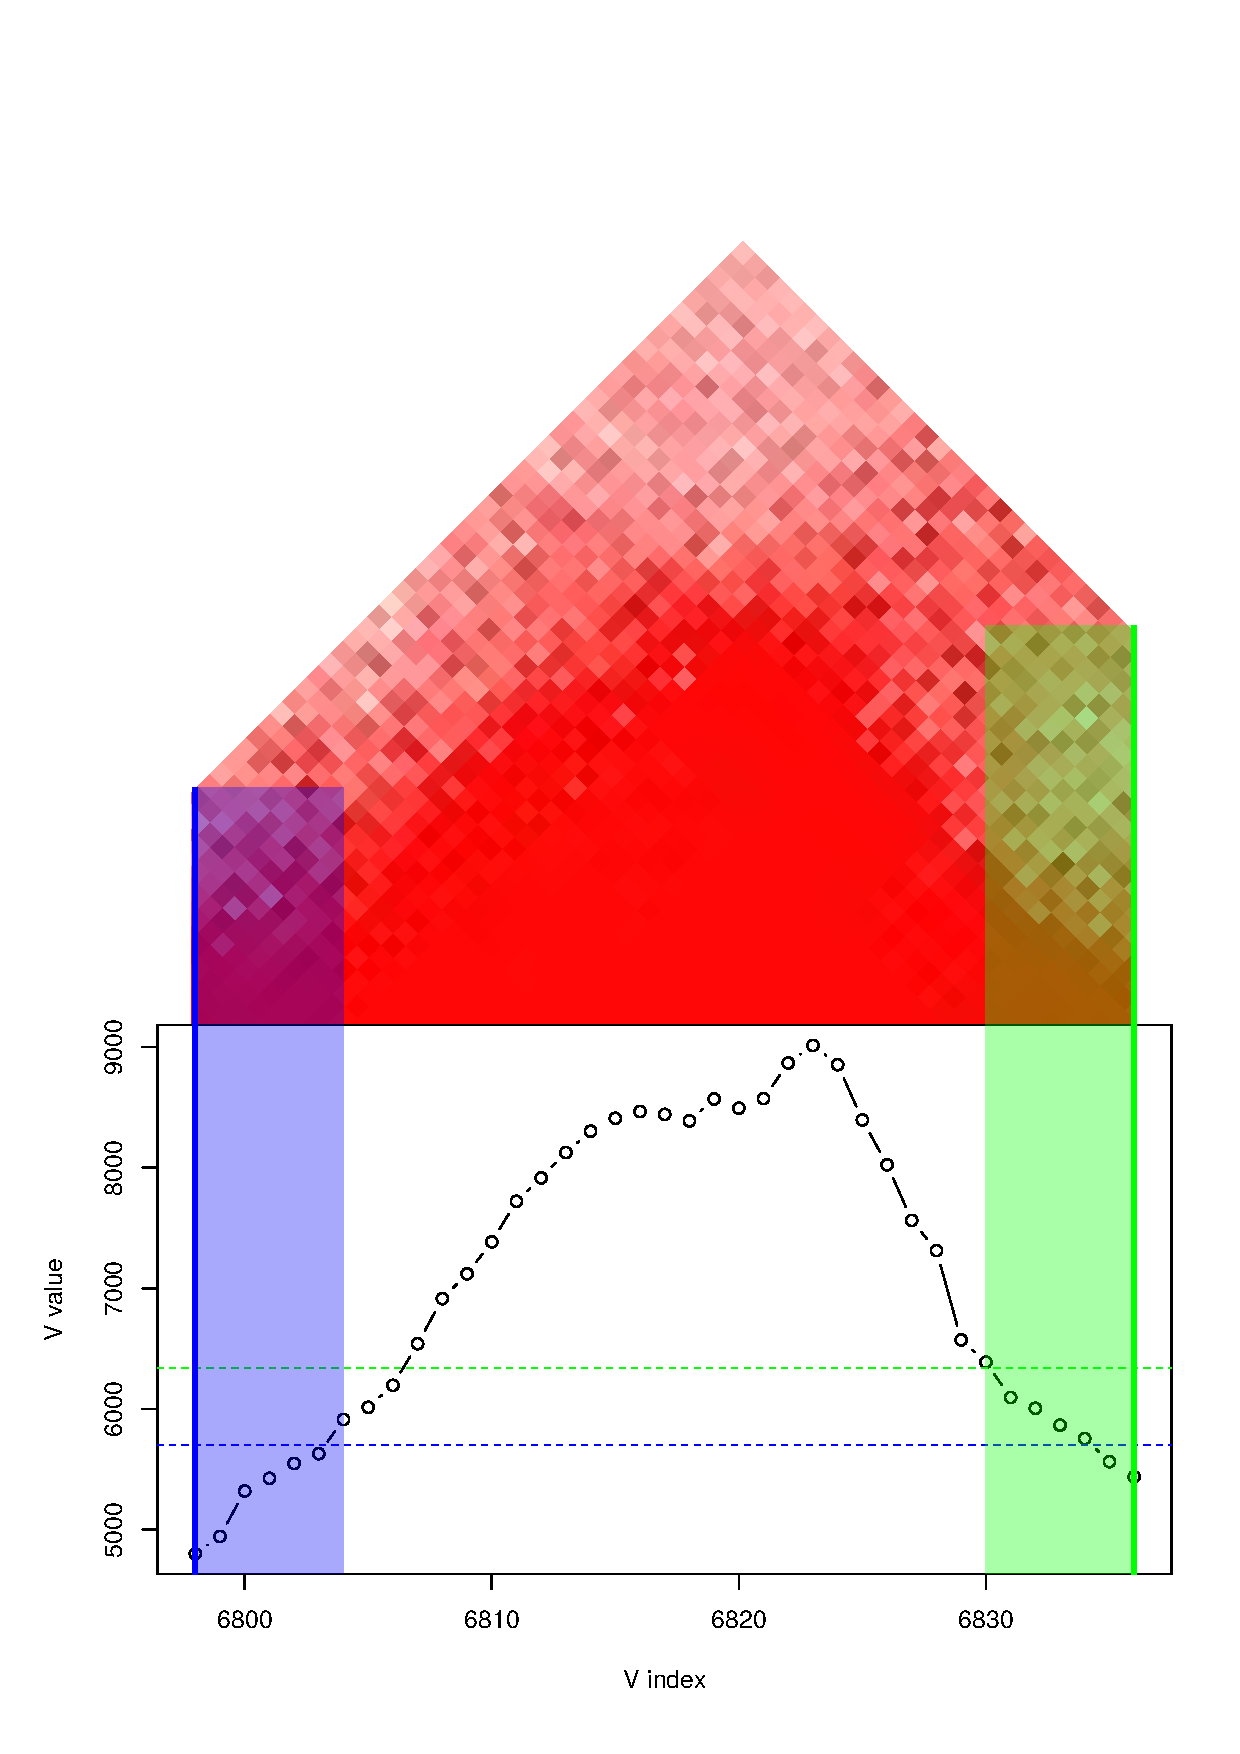
\includegraphics[width=0.7\textwidth]{Figures/5_boundary_example.pdf}
	\caption{Example of the calculated sums of interactions through a TAD, how boundaries were extended until they reach the threshold and the corresponding TAD in the Hi-C matrix, visualized in Juicebox. The solid vertical lines represent the TAD borders, the horizontal dashed lines represent the threshold required to stop extending boundaries and the transparent areas represent the final boundaries. All blue elements relate to the left side, while all green elements relate to the right side.}
	\label{boundary_ex}
\end{figure}

\begin{figure}[ht]
	%\centering
	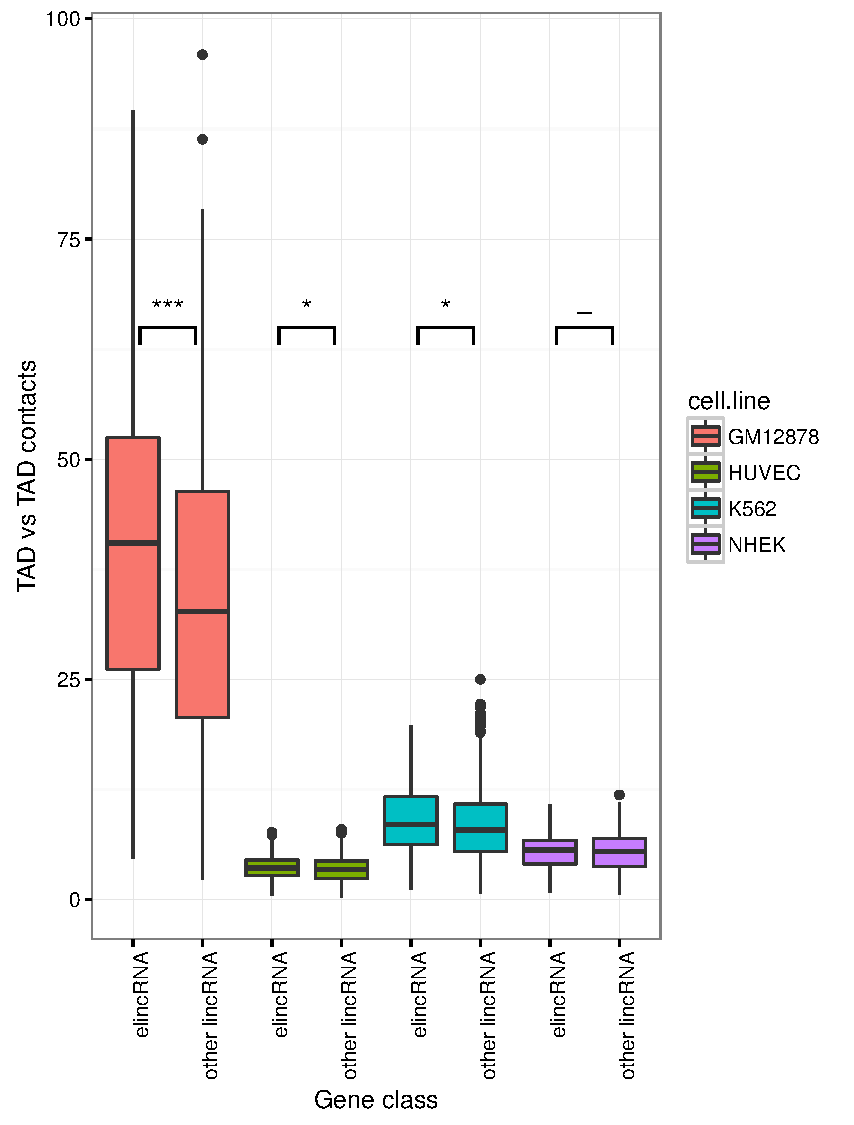
\includegraphics[width=0.7\textwidth]{Figures/6_TAD_TAD_contact.pdf}
	\caption{Mean amount of DNA:DNA contact within TADs for elincRNAs compared to other lincRNAs across different cell lines. Set of genes as defined in GM12878 are used for all comparisons. Two tailed Mann-Whitney test, $***P<0.001; *P<0.05$; $-$ non-significant}
	\label{TAD_TAD_contacts}
\end{figure}

\begin{figure}[ht]
	%\centering
	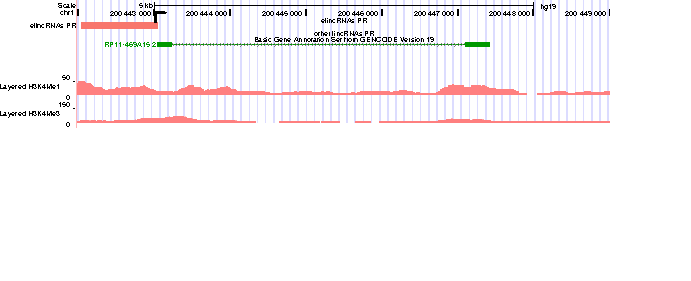
\includegraphics[width=1\textwidth]{Figures/7_merged_examples.pdf}
	\caption{Genome browser view showing an example of an elincRNA (putative promoter region in pink, bottom) and two other lincRNAs (putative promoter region in blue, top). The promoter regions of other lincRNAs have low levels of promoter (H3K4Me3) and enhancer (H3K4Me1) histone marks, while the promoter region of the elincRNA has high H3K4Me1, but low H3K4Me3. Gene bodies are depicted in green, with solid boxes as exons and thin lines as introns.}
	\label{Genome_browser}
\end{figure}
\FloatBarrier
\section*{Discussion}

Although it has been long recognized that conformation of chromatin is key in the regulation of gene transcription programs, features that underlie transcriptional regulation mechanisms of chromatin organization remain relatively unclear \cite{Bonev2016}⁠. Following the development of chromosome conformation capture techniques over a decade ago \cite{Dekker2002}⁠, advances in other 3C-based technologies have allowed the quantification of chromosomal interaction frequencies between genomic loci in close proximity, both locally (i.e. 3C and 4C) and genome-wide (i.e. Hi-C and ChIA-PET) \cite{Dekker2013}.

LincRNAs originated from enhancers (elincRNAs) have been shown to modulate chromosomal architecture \cite{Yin2015}⁠ and are frequently located within topologically associated domains (TADs) associated with high levels of genomic interactions (Tan et al, 2016, under revision). Here, I used publicly available genomic data to investigate the prevalence of elincRNAs regulation in modulating chromosomal architecture. Together with strong enrichment of cohesin binding at elincRNAs promoter regions and their frequent localization at loop anchors, the high amount of intra-TAD contacts associated with elincRNAs support their putative role in regulating enhancer-promoter loops. 

There is ongoing debate on the biological relevance of elincRNA transcription as to whether their associated functional roles are transcript- or transcription-dependent. Notably, the association between elincRNAs and chromosomal organization does not constitute a proof for their role in promoting contact, as it might be a consequence of the presence of active enhancers at their promoter region, rather than the elincRNA transcript itself. A good way to strengthen the hypothesis would be to perform similar analysis by comparing active enhancers producing elincRNAs with other active enhancers producing unstable bidirectionally-transcribed eRNAs. Ultimately, to dissect the molecular mechanisms underlying these enhancer-associated regulation of chromosomal conformation requires genetic manipulation of elincRNA transcript abundance, for example by using RNAi and inhibiting their transcription with CRISPR-Cas9 \cite{Li2013}⁠.

Furthermore, extending the analysis from intra-topological domain interactions to between-TAD contacts \cite{Fraser2015}⁠, inter-chromosomal contacts, and eventually association with nuclear lamina would provide a more complete overview of chromosomal interactions that shape the nuclear architecture. These analyses could also be performed on different cell-lines to reveal if the effect of elincRNAs in nuclear architecture is cell-line specific, or more generalized. 

The current resolution of global chromosomal conformation capture techniques (including Hi-C) remains a limiting factor in measuring accurate interaction frequencies as it is impossible to look at contacts between elincRNAs that are smaller than the highest resolution (1-5 Kb) \cite{Rao2014}⁠. Instead, only an estimation of the region surrounding the gene can be measured. In addition, even at high contact resolutions, bulk Hi-C data can only provide an average estimate of all chromosomal contacts happening in a cell population, thus masking the dynamics and cell-to-cell variablilities in contacts. Recently, a single-cell Hi-C protocol has been developed \cite{Nagano2013}⁠, allowing one to examine DNA contacts profiles at a single cell resolution. Indeed, such single cell techniques, combined with a higher contact resolution, would provide much more power to shed light on the impact of elincRNAs on gene expression regulation through modulating chromosome architecture.

\section*{Materials and methods}
Unless stated otherwise, all statistical tests were performed using R 3.3.1 \cite{RCoreTeam2016}⁠. Overlapping of genomic elements were done using either bedtools 2.26 \cite{Quinlan2010}⁠or the “intervals” package \cite{Bourgon2015}⁠ in R. Manipulations on Hi-C contact matrices were performed using the “Matrix” package \cite{Bates2016}⁠.

\subsection*{elincRNA definition}

LincRNAs and protein-coding genes sets were provided by Tan et al (2016, under revision). Those sets were obtained using data from the ENCODE website. The list of genes used in all analyses corresponds to genes expressed in the GM12878 human lymphoblastoid cell line. Subcategories of genes were defined based on overlap between their putative promoter region, defined as the 1kb region upstream from the transcription start site and predicted regulatory elements available on ENCODE \cite{ENCODEProject2012}⁠. These regulatory elements are predicted computationally from histone marks by a hidden Markov-model. Predicted active promoters and all enhancers were considered. The 2 categories of lincRNAs that are used throughout this report are elincRNAs, defined as overlapping enhancers marks but no promoters marks in their putative promoter region, and other lincRNAs defined as overlapping neither enhancer nor promoters marks in their promoter region (Figure \ref{Genome_browser}).



\subsection*{TAD definition}

The list of TADs used in the computations is based on that from \cite{Rao2014}. They called the TADs based on Hi-C data across different human cell lines, normalized and processed with their own protocol. Here, all the large TADs that completely encompass smaller ones were removed to preserve the signal from the boundaries of the small TADs. Boundaries from very large TADs would otherwise contain the signal from smaller TADs inside, generating noise.

\subsection*{Hi-C data and normalization}

Contacts were calculated using Hi-C contact matrices from \cite{Rao2014}. All computations are performed on 5kb resolution matrices constructed from all read pairs mapping to the genome with a MAPQ score of at least 30. The matrices were normalized using the KR normalization vector provided by the authors whenever possible. SQRTVC (square root vanilla coverage) was used for chromosome 9 of all cell lines, because the KR algorithm did not converge for chromosome 9 of K562 probably as a result of the high sparsity of the matrix. I chose SQRTVC as a substition for KR as the authors reported this method  to yield very close results to KR. 
The normalization procedure consists in dividing each entry in the contact matrix M by a corresponding value in the normalization vector N:

\vspace{0.2in}
$M^*_{i,j}=\frac{M_{i,j}}{N_{KR}[\frac{i}{res}]*N_{KR}[\frac{j}{res}]}$
\vspace{0.2in}

\noindent Where $M_{i,j}$ is an entry from the raw matrix and $M^*_{i,j}$ corresponding normalized entry.

\subsection*{TAD boundaries definition}

Boundaries are extended from TAD borders towards the interior of TADs using a custom algorithm. The method used to define boundaries relies on the assumption that boundaries are insulated regions. In other words, there are few interactions between elements located before and those after the boundaries. The insulation is measured by sliding a diamond (Figure \ref{interact_hic}A) on every position along the matrix diagonal and computing the sum in the diamond at each position. Lower values represent more insulated regions. The size of the diamond has been set to an arbitrary threshold of 100kb, considered reasonable as the median length of filtered TADs is 140kb. 
More formally, the algorithm can be described as sliding a diamond of width w  along the diagonal of a square matrix M of n dimensions on all positions d between w and n-(w-1). Those latter limits are set to prevent the diamond from getting out of the matrix. At each position, the sum of all values in the diamond is stored in a vector V. This can be rewritten as: 

\vspace{0.2in}
$\left\{\begin{matrix}1\leq w\leq \frac{n}{2}+1 \\ \forall d\in\left \{ w , ... , n-\left ( w-1 \right ) \right \}\end{matrix}\right. V_{d}=\sum_{i=d-(w-1)}^{d}\sum_{j=d}^{d+(w-1)}M_{i,j}$
\vspace{0.2in}

\noindent The sums from the diamond are then used to compute boundaries. For all TADs, boundaries are extended inwards from the borders as long as the value of V does not exceed an arbitrary threshold defined as the starting value (at the border) plus 10\% of the maximum value in the TAD (Figure \ref{boundary_ex}).

\subsection*{Conservation and tissue specificity}

The sequence conservation was previously calculated in exons (Tan et al, 2016, under revision) through mammalian and primate evolution using phastCons scores \cite{Siepel2005}⁠ and averaged phastCons score were used as a measure of exonic sequence conservation. Tissue specificity index ($\tau$) was computed following the described procedure in \cite{Kryuchkova2015a}, considering only genes with expression above a cutoff of 0.1 RPKM.

\subsection*{Expression levels}

Processed median expression data for elincRNAs and protein-coding genes in 4  different cell lines were calculated by Tan et al, 2016, under revision. The original data comes from ENCODE \cite{ENCODEProject2012}.

\subsection*{DNA:DNA contacts}

For each gene overlapping a TAD, the mean contact inside the respective TAD was used as a measure. For single genes that overlap several TADs, the contacts are computed for each TAD independently. The mean contact in a TAD is computed by taking the arithmetic mean of all values in a square submatrix spanning from the beginning to the end of the TAD in the intrachromosomal matrix (Figure \ref{interact_hic}B).

\subsection*{Chip-seq data}

Chip-seq peaks for CTCF, RAD21 and SMC3 in GM12878 were retrieved from the ENCODE website \cite{ENCODEProject2012}⁠. Cohesin peaks were defined as the union between the peaks of RAD21 and SMC3 subunits. The CTCF and cohesin exclusive peaks were obtained by using the intersect and subtract tools from the bedtools suite.

\subsection*{Enrichment of genetic elements}

All enrichment tests were performed using the genome association tester (GAT) \cite{Heger2013}⁠ version 1.2. This program allows to test if genomic segments of interest are found in a desired set of annotations more often than expected if they were distributed randomly in a workspace. All tests using lincRNAs as annotations or segments were performed using the intergenic regions of the human genome as a workspace. When testing for enrichment of anchors at boundaries, the whole genome was used as the workspace. For all tests, the number of samples was set to 10,000, the number of buckets was consequently adjusted to 270,000 and segments overlap was used as the measure.

For all enrichment tests, two values are reported in the results section: Fold enrichment and q-value. The fold enrichment corresponds to the ratio of observed to average expected number of segments overlapping the given annotation, it is higher than 1 if the segment is enriched compared to random expectation, and lower than 1 if the segment is depleted. The q-value corresponds to the p-value once it has been corrected for multiple testing using false discovery rate controlled with the Benjamin-Hochberg procedure.

\section*{Acknowledgements}
I wish to thank Jennifer Yihong Tan for her precious advices and help throughout the project and writing of the report. I also wish to thank Ana Claudia Marques for her suggestions, general guidance and corrections in the report. Finally, I want to thank Adam Alexander Thil Smith for  his help with technical issues and code optimization and Maria Ferreira da Silva for her suggestions and critical reading of the report.
Computationally demanding analysis were performed at the Vital-IT Center for High Performance Computing of the Swiss Institute of Bioinformatics (www.vital-it.ch).

%\bibliography{First_step}{}
\bibliographystyle{apalike}
\fancyhead[L]{\slshape }
\bibliography{firststep}
\end{document}